% ============================================================================
% Elective Surgery Scheduling -- Executive Beamer Deck
% Primary model: interval-based Constraint Programming (Google OR-Tools
% CP-SAT). A day-bucket MILP (OR-Tools/CBC, optionally Gurobi) is kept only
% as the comparison point that justifies that choice; Hexaly is an optional,
% license-gated extension. Mirrors FORMULATION.md and RESULTS.md in the
% repository -- same notation, same numbers.
%
% Compile with: pdflatex or xelatex (run twice for the table of contents).
%   pdflatex or_surgery_scheduling_beamer.tex
% ============================================================================
\documentclass[aspectratio=169]{beamer}

\usetheme{Madrid}
\usecolortheme{default}

\usepackage[utf8]{inputenc}
\usepackage[T1]{fontenc}
\usepackage{amsmath,amssymb}
\usepackage{booktabs}
\usepackage{array}
\usepackage{graphicx}
\usepackage{hyperref}
\usepackage{xcolor}

\definecolor{hospitalblue}{RGB}{0,70,120}
\definecolor{overdue}{RGB}{180,30,30}
\definecolor{ok}{RGB}{20,120,60}
\setbeamercolor{structure}{fg=hospitalblue}
\setbeamertemplate{navigation symbols}{}
\setbeamerfont{footnote}{size=\tiny}

\title{Elective Surgery Scheduling}
\subtitle{An Interval-Based Constraint Programming Model\\
\small Google OR-Tools CP-SAT (primary) $\cdot$ MILP comparison (CBC/Gurobi) $\cdot$ Hexaly (optional)}
\author{Operations Research Case Study}
\date{\today}

\begin{document}

% ----------------------------------------------------------------------------
\begin{frame}
  \titlepage
\end{frame}

\begin{frame}{Roadmap}
  \tableofcontents
\end{frame}

% ============================================================================
\section{The Case}
% ============================================================================

\begin{frame}{The Case, in One Slide}
  \textbf{A large hospital group} needs to decide, for every elective surgical case on
  its waiting list:
  \begin{itemize}
    \item \textbf{Which procedure} runs \textbf{in which operating room}, \textbf{at
      what time}
    \item \textbf{On which day}, across a \textbf{one-week} planning horizon
    \item \textbf{With which surgeon}
    \item And, since not everything fits this week: \textbf{which cases wait}
  \end{itemize}
  \vfill
  \textbf{What we were asked for (two deliverables):}
  \begin{enumerate}
    \item A problem formulation: sets, parameters, decision variables, objective,
      constraints, \emph{and the assumptions behind them} -- in actual math. We choose
      what to include and exclude, and say why.
    \item A working demo solver: small data, runnable Python, produces a schedule.
      Plain terminal output or a simple image is enough.
  \end{enumerate}
  \vfill
  \textit{We were explicitly invited to simplify and to ground choices in evidence
  (papers, real data, industry pain points) -- and explicitly told this should stay
  small: ``a well-reasoned model with a small demo beats an exhaustive one.''}
\end{frame}

\begin{frame}{Why This Is Hard -- and Why It Matters}
  \begin{columns}[T]
    \begin{column}{0.55\textwidth}
      \textbf{The bottleneck is real, and documented:}
      \begin{itemize}
        \item Portugal's SIGIC system: of $\sim$7{,}400 waiting-list patients audited in
          2016, \textbf{16\% had already breached} their clinical maximum-wait deadline,
          by an average of \textbf{147 days} (Marques \& Captivo, 2015).
        \item The UK NHS Referral-to-Treatment framework and Canadian provincial
          wait-time benchmarks track the same kind of breach rate, for the same reason.
        \item Cardoen, Demeulemeester \& Beli\"en (2010): \emph{the} literature review
          for this problem family -- classifies it, doesn't solve one country's
          instance of it.
      \end{itemize}
    \end{column}
    \begin{column}{0.45\textwidth}
      \textbf{NP-hard, structurally:}
      \begin{itemize}
        \item Room-capacity feasibility alone reduces to bin packing.
        \item Add tiered priority, surgeon limits, shared equipment, and downstream
          beds, and the \emph{choice of solver paradigm} -- not just the solver
          brand -- is the central technical decision in this deck.
      \end{itemize}
    \end{column}
  \end{columns}
  \vfill
  \footnotesize Evidence used to \emph{justify the model's shape} (priority + waiting
  time + escalating penalty) -- not as a literal country-specific subject. Every
  numeric value is an instance-level, overridable parameter in the code.
\end{frame}

% ============================================================================
\section{Why Constraint Programming, Not a Bigger MILP}
% ============================================================================

\begin{frame}{The Central Modeling Decision}
  A linear capacity-sum constraint (``total minutes used this day $\le k$'') only
  certifies that a set of durations \emph{fits} -- not that they can be placed
  \emph{without colliding}. For a single room those coincide. They stop coinciding the
  moment a resource is \textbf{shared across rooms} -- a surgeon in two rooms, one
  imaging unit serving two rooms:
  \begin{itemize}
    \item A surgeon's daily-minutes \emph{sum} can be within limit while two of their
      cases, in two rooms, are scheduled to overlap -- physically impossible, invisible
      to a sum.
    \item A shared device's day-count cap can be \emph{needlessly tighter} than
      reality: it forbids two genuinely non-overlapping uses a real device could serve
      back-to-back.
    \item A day-bucket model has \textbf{no correct way to express} a multi-day
      recovery-bed stay that starts on the day of surgery -- a constraint the case
      prompt names directly.
  \end{itemize}
  \vfill
  \footnotesize RESULTS.md shows this is not theoretical: a comparison MILP run on the
  same data finds a schedule that is forbidden outright by its own day-bucket
  equipment constraint, even though a strictly better, legal one exists.
\end{frame}

\begin{frame}{Why CP-SAT, Specifically}
  \textbf{The textbook MILP alternative} -- a disjunctive big-M formulation, one binary
  ``A-before-B'' variable per potentially-conflicting case pair -- works, but
  (Baptiste, Le Pape \& Nuijten, \emph{Constraint-Based Scheduling}, 2001):
  is quadratic in the number of conflicting pairs, and resource \emph{sharing}
  (capacity $>1$) needs combinatorially more pairs still.
  \vfill
  \texttt{NoOverlap} / \texttt{Cumulative} are \textbf{global constraints with their
  own polynomial propagation}: \texttt{NoOverlap} via Vil\'im's $O(n\log n)$
  Theta-tree sweep (2004); \texttt{Cumulative} via timetabling + edge-finding (Schutt,
  Feydy, Stuckey \& Wallace, CP 2009). They prune the search tree directly from
  temporal structure, instead of the solver \emph{discovering} it case-pair by
  case-pair through branching.
  \vfill
  \textbf{CP-SAT's engine:} a parallel portfolio of complete-search workers plus Large
  Neighbourhood Search workers sharing learned clauses (Perron \& Furnon, OR-Tools
  docs) -- which is why we don't hand-write a custom search strategy, and why we
  \emph{do} warm-start it from a fast greedy heuristic's assignment
  (\texttt{model.AddHint(...)}; discrete assignment only, never exact clock times).
\end{frame}

% ============================================================================
\section{Scope, Assumptions \& What's Excluded}
% ============================================================================

\begin{frame}{Assumptions -- Stated, Not Hidden}
  \begin{enumerate}
    \footnotesize
    \item \textbf{Deterministic durations} -- one estimate per case (e.g. historical
      median); standard tractable approximation (Denton et al., 2010); stochastic
      extension named, not attempted, to keep this demo small.
    \item \textbf{Fixed turnover/cleaning buffer}, added to every case's room-occupation
      interval -- not modeled as a separate sequence-dependent activity.
    \item \textbf{Surgeons are the binding staffing resource}; nurses/anaesthetists
      assumed pre-rostered to the room.
    \item \textbf{One occurrence per patient per week} -- conservative default.
    \item \textbf{Recovery/ICU beds modeled, with a constant-capacity caveat:} bed
      \emph{capacity} is constant across the week; day-varying capacity would need a
      segmented version (flagged, not silently assumed away).
    \item \textbf{One ad hoc institutional rule, as a worked example} -- a configurable
      ``pediatric block'' carve-out, to show such rules cost nothing structurally.
    \item \textbf{Single week, no same-day disruption.} An offline weekly plan -- not a
      reactive re-scheduler for an emergency walking in mid-day. Named explicitly as
      the most valuable next extension (Roadmap), not folded in here.
  \end{enumerate}
\end{frame}

\begin{frame}{What's In, What's Out -- and Why}
  \footnotesize
  \begin{columns}[T]
    \begin{column}{0.5\textwidth}
      \textbf{\textcolor{ok}{Included}}
      \begin{itemize}
        \item Priority + waiting-time penalty (evidence-based, multi-system)
        \item Exact room/surgeon timing (no double-booking, not just a budget)
        \item Surgeon daily/weekly limits
        \item Room-service roster, pediatric-block worked example
        \item Exact shared-equipment concurrency
        \item Downstream recovery/ICU beds (case prompt names this directly)
      \end{itemize}
    \end{column}
    \begin{column}{0.5\textwidth}
      \textbf{\textcolor{overdue}{Excluded, named explicitly}}
      \begin{itemize}
        \item Stochastic durations -- top extension, not attempted here
        \item Same-day / real-time re-optimization -- a different problem
        \item Nurses/anaesthetists as separate resources
        \item Sequence-dependent (vs. constant) turnover time
        \item Patient day-of-week preference
        \item Multi-week rolling horizon
      \end{itemize}
    \end{column}
  \end{columns}
\end{frame}

% ============================================================================
\section{The Model}
% ============================================================================

\begin{frame}{Sets and Parameters}
  \footnotesize
  \begin{table}
    \centering\tiny
    \begin{tabular}{cl}
      \toprule
      Symbol & Description \\
      \midrule
      $c \in C$, $d \in D=\{1,\ldots,5\}$, $r \in R$, $h \in H$, $e \in E$ & Cases, days,
        rooms, surgeons, shared equipment \\
      $D_c \subseteq D$ & Days case $c$ may run ($\{1\}$ if priority 4, else $D$) \\
      $t_c^{\text{op}}$, $t_c^{\text{clean}}$, $t_c^{\text{tot}}$ & Operative / cleaning
        / total room time for case $c$ \\
      $k_{dr}$, $k_{hd}$, $k_h$ & Room capacity; surgeon daily / weekly time limit \\
      $a_{dr}^{s}\in\{0,1\}$ & 1 if room $r$ on day $d$ is rostered to service $s$ \\
      $p_c \in \{1,2,3,4\}$, $dd_c$, $\mu_p$, $\alpha$, $w_c$ & Priority; slack to
        deadline; penalty multiplier; urgency mult.; non-scheduling weight \\
      $u_{ce}\in\{0,1\}$, $\kappa_{ed}$ & Equipment $e$ required by case $c$; capacity
        of $e$ on day $d$ \\
      $\rho(c)$, $\text{los}_c$, $\beta_\rho$ & Bed pool needed; length of stay; bed
        count for pool $\rho$ \\
      \bottomrule
    \end{tabular}
  \end{table}
  Every default above is an instance-level, overridable field on
  \texttt{PlanningInstance} -- not a hard-coded constant.
\end{frame}

\begin{frame}{Decision Variables and Objective}
  \footnotesize
  For every $(c,d,r)$ surviving the eligibility pre-filter (room-service roster,
  ambulatory-only, pediatric block, surgeon availability):
  \[
    \text{pr}_{cdr}\in\{0,1\},\quad \text{start}_{cdr},\,\text{end}_{cdr}\in[0,k_{dr}],
    \quad \text{iv}_{cdr}=\texttt{NewOptionalIntervalVar}(\text{start}_{cdr},\,t_c^{\text{tot}},\,\text{end}_{cdr},\,\text{pr}_{cdr})
  \]
  and, for every non-priority-4 case, $u_c\in\{0,1\}$ with $\sum_{d,r}\text{pr}_{cdr}+u_c=1$.
  \vfill
  \[
    \min \;
    \underbrace{\sum_{c:\,dd_c \ge 0}\ \sum_{d,r} \big[dd_c + d\big]\, \text{pr}_{cdr}}_{\text{on-time, prefer earlier days}}
    \;+\;
    \underbrace{\sum_{c:\,dd_c < 0}\ \sum_{d,r} \big[dd_c + \alpha d\big]\, \text{pr}_{cdr}}_{\text{overdue, urgency mult. }\alpha}
    \;+\;
    \underbrace{\sum_{c:\,p_c \ne 4} p_c\, w_c\, u_c}_{\text{non-scheduling penalty}}
  \]
  \[
    w_c = \text{PenaltyCurve}\big(dd_c \cdot \mu_{p_c}\big) + 1.2 \cdot \max_{c'\in C} dd_{c'}
    \quad \text{(calibrated to dominate Terms 1--2)}
  \]
\end{frame}

\begin{frame}{Constraints I -- Case Disposition \& Eligibility}
  \footnotesize
  \textbf{C1} -- at most one occurrence per patient per week:
  $\sum_{c:\text{patient}(c)=n} \sum_{d,r} \text{pr}_{cdr} \le 1\ \forall n$.\quad
  \textbf{C2} -- priority-4 cases must run on day 1:
  $\sum_r \text{pr}_{c,1,r} = 1\ \forall c: p_c=4$.\quad
  \textbf{C3} -- every other case scheduled exactly once, or penalised:
  $\sum_{d,r} \text{pr}_{cdr} + u_c = 1$.
  \vfill
  \textbf{C4--C6 (pre-filter, not separate rows):} room-service roster
  ($a_{dr}^{\,\text{service}(c)}=0 \Rightarrow$ no candidate); ambulatory-only rooms
  admit only day-case scopes; pediatric block forbids age $>i^\dagger$ in service
  $s^\dagger$'s rooms on day $d^\dagger$.
  \vfill
  \textit{These three eliminate infeasible $(c,d,r)$ triples before the model is even
  built -- the same effect as a constraint row, at a fraction of the variable count.}
\end{frame}

\begin{frame}{Constraints II -- Capacity \& Shared Resources}
  \footnotesize
  \textbf{C7 -- room capacity, exact:} $\texttt{AddNoOverlap}(\{\text{iv}_{cdr}: d,r
  \text{ fixed}\})$.\quad
  \textbf{C8 -- surgeon, exact + daily cap:}
  $\texttt{AddNoOverlap}(\{\text{iv}_{cdr}:\text{surgeon}(c)=h, d \text{ fixed}\})$
  \emph{plus} $\sum_{c} t_c^{\text{op}}\text{pr}_{cdr} \le k_{hd}$.\quad
  \textbf{C9 -- surgeon weekly limit:} $\sum_{d,r} t_c^{\text{op}}\text{pr}_{cdr} \le k_h$.
  \vfill
  \textbf{C10 -- shared equipment, exact concurrency:}
  \[
    \texttt{AddCumulative}\big(\{\text{iv}_{cdr}: u_{c,e}=1, d \text{ fixed}\},\,
    \text{demands}=1,\, \text{capacity}=\kappa_{ed}\big)
  \]
  \textbf{C11 -- downstream recovery/ICU beds:}
  \[
    \text{bed}_c=\texttt{NewOptionalIntervalVar}(\text{dayof}_c,\,\text{los}_c,\,
    \text{dayof}_c+\text{los}_c,\,\text{is\_scheduled}_c),\quad
    \texttt{AddCumulative}(\{\text{bed}_c:\rho(c)=\rho\},\,1,\,\beta_\rho)
  \]
  \vfill
  \textit{C7--C11 share one interval per candidate slot -- a case's start propagates
  across every resource it touches without an explicit channeling constraint.}
\end{frame}

\begin{frame}{Alternative Formulations Considered}
  \footnotesize
  \textbf{A day-bucket MILP} (\texttt{milp\_baseline\_solver.py}, OR-Tools/CBC,
  optionally Gurobi) was also built -- same C1--C6, C9; C7/C10 as linear sums instead of
  \texttt{NoOverlap}/\texttt{Cumulative}; no C11 (can't express a multi-day bed stay
  correctly without intervals). It exists \textbf{purely as the empirical comparison
  that justifies the CP-SAT choice} -- not a second deliverable. Results next section.
  \vfill
  \textbf{Hexaly} (\texttt{hexaly\_solver.py}) is a real, non-stub local-search
  integration, written against a set-partition encoding -- an \textbf{optional, future
  contribution}: no academic license was available while building this, so it runs
  only as a graceful fallback to the MILP above today, with setup instructions printed
  at runtime. Pointed at as the natural backend for very large instances or real-time
  re-optimization, not benchmarked here.
\end{frame}

% ============================================================================
\section{Results}
% ============================================================================

\begin{frame}{Results -- Demo Instance (20 cases, 5 rooms, 6 surgeons)}
  \footnotesize
  \begin{table}
    \centering
    \begin{tabular}{lccccc}
      \toprule
      Solver & Status & Objective & Gap & Scheduled & Time \\
      \midrule
      Greedy & Feasible & 163.0 & -- & 20/20 & 0.000s \\
      \textbf{CP-SAT (primary)} & \textbf{Optimal} & \textbf{155.0} & 0.00\% & 20/20 & 0.10s \\
      OR-Tools/CBC (comparison MILP) & Optimal & 157.0 & 0.00\% & 20/20 & 0.03s \\
      Gurobi (comparison MILP) & Optimal & 157.0 & 0.00\% & 20/20 & 0.06s \\
      Hexaly ($\to$ CBC fallback) & Optimal & 157.0 & 0.00\% & 20/20 & 0.02s \\
      \bottomrule
    \end{tabular}
  \end{table}
  \vfill
  \normalsize\textbf{CP-SAT wins on objective (155 vs.\ 157), not by searching harder,
  but by modeling the shared C-arm correctly:} \texttt{AddCumulative} checks literal
  time overlap, so it legally places two C-arm cases on Tuesday, in different rooms,
  at non-overlapping times -- a schedule the MILP's day-count cap forbids outright.
\end{frame}

\begin{frame}{Results -- Medium Instance (200 cases, 12 rooms, 17 surgeons)}
  \footnotesize 60-second budget per solver.
  \begin{table}
    \centering\footnotesize
    \begin{tabular}{lccccc}
      \toprule
      Solver & Status & Objective & Gap & Scheduled & Time \\
      \midrule
      Greedy & Feasible & 70{,}883.0 & -- & 124/200 & 0.00s \\
      \textbf{CP-SAT (primary)} & Feasible & \textbf{41{,}548.0} & 4.30\% & \textbf{130/200} & 60.45s \\
      OR-Tools/CBC (comparison MILP) & Feasible & 44{,}346.0 & 0.31\% & 128/200 & 60.11s \\
      Gurobi (comparison MILP) & Feasible & 44{,}333.0 & 0.45\% & 129/200 & 1.65s \\
      Hexaly ($\to$ CBC fallback) & Feasible & 44{,}346.0 & 0.31\% & 128/200 & 60.13s \\
      \bottomrule
    \end{tabular}
  \end{table}
  \vfill
  \textbf{The demo's effect reproduces, larger, at scale:} CP-SAT's objective is
  \textbf{6.3\% lower} (41{,}548 vs.\ 44{,}346) while scheduling \textbf{2 more cases},
  even though its own gap (4.30\%) looks less converged than CBC's (0.31\%).
\end{frame}

\begin{frame}{Reading This Correctly}
  \footnotesize
  \begin{itemize}
    \item \textbf{A tighter own-gap is not a better answer.} CBC's 0.31\% gap is tight
      because its feasible region is \emph{smaller} -- a day-bucket relaxation that
      structurally excludes schedules CP-SAT can reach. It's easier to prove there's
      nothing better than 5 in $\{1,\ldots,5\}$ than in $\{1,\ldots,100\}$; that doesn't
      make 5 the better answer.
    \item \textbf{Same mechanism at both scales.} The 20-case C-arm story and the
      200-case 6.3\%/+2-cases result are the same effect: exact temporal/resource
      reasoning recovers schedules a coarser aggregate constraint forbids outright.
    \item \textbf{This is why CP-SAT is the primary deliverable}, with the MILP kept
      only as the comparison that makes the claim falsifiable and, here, confirmed.
  \end{itemize}
  \vfill
  \begin{table}
    \centering\tiny
    \begin{tabular}{lcc}
      \toprule
       & CP-SAT (primary) & MILP (comparison) \\
      \midrule
      Exact timing/overlap & \textbf{yes} & no \\
      Exact equipment concurrency & \textbf{yes} & no (day-count) \\
      Downstream beds (C11) & \textbf{yes} & not expressible \\
      License & free & free (CBC) / commercial (Gurobi) \\
      \bottomrule
    \end{tabular}
  \end{table}
\end{frame}

% ============================================================================
\section{Visual Schedule}
% ============================================================================

\begin{frame}{Demo Instance -- Primary CP-SAT Model}
  \centering
  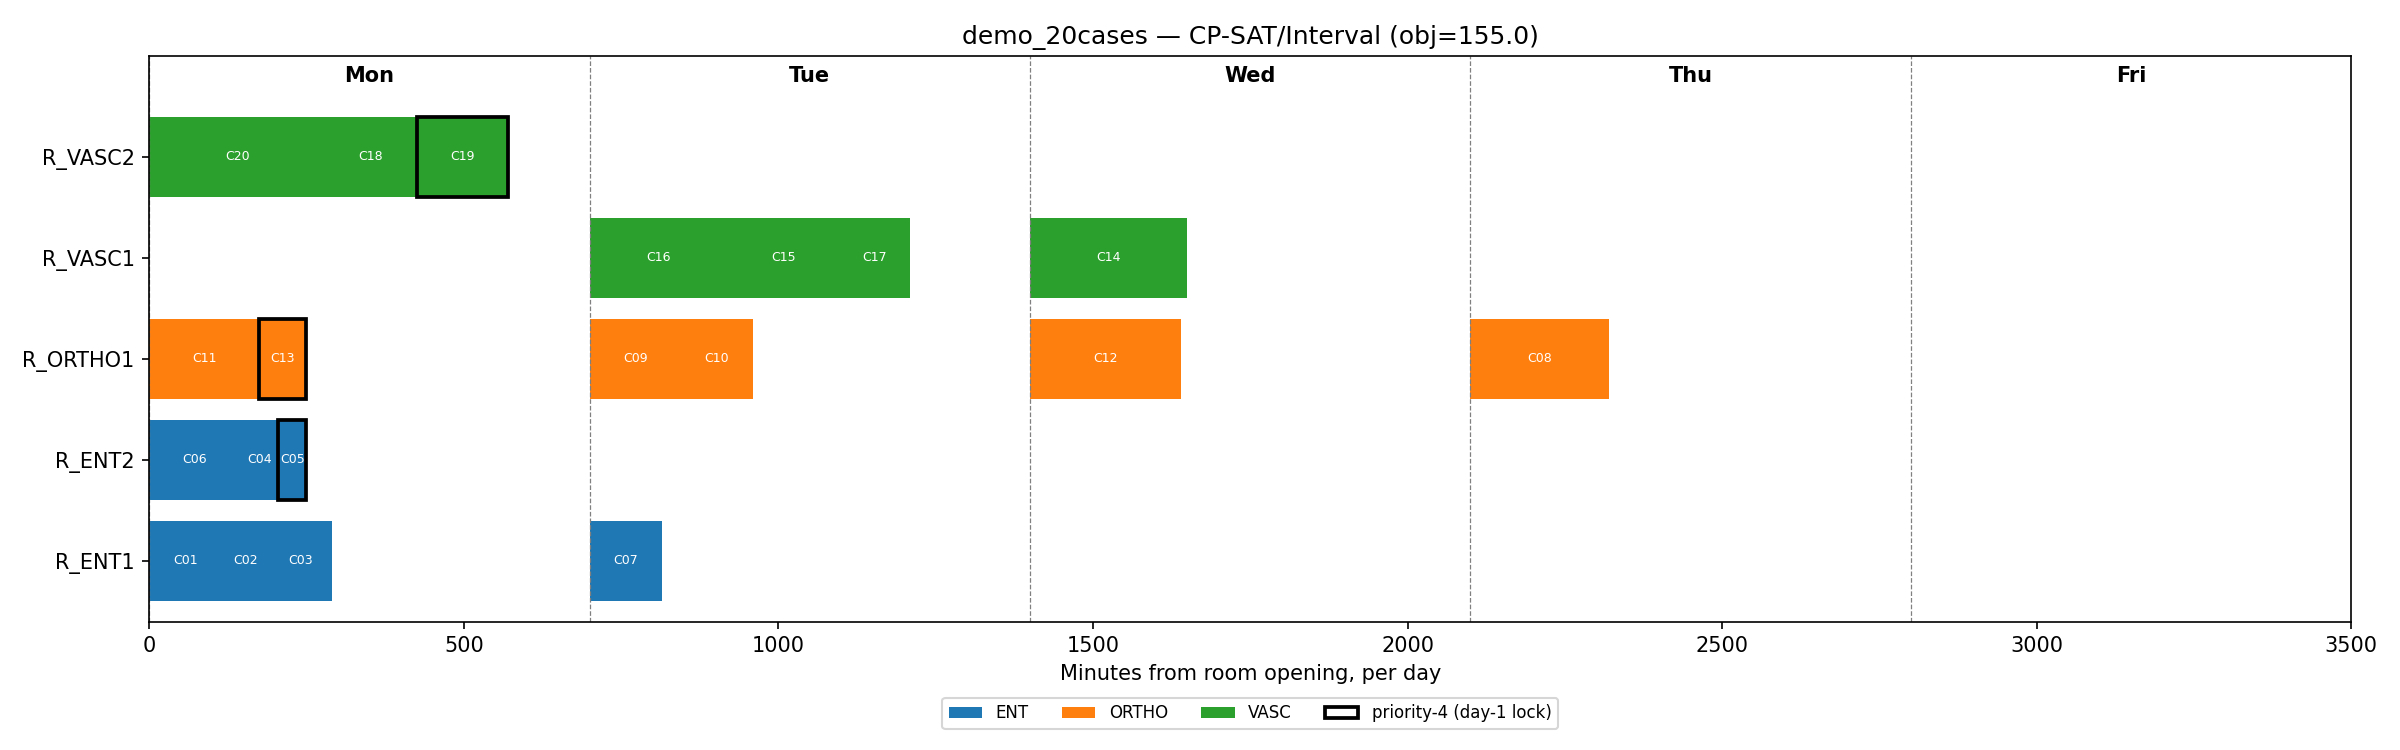
\includegraphics[width=\textwidth]{img/demo_cp_sat.png}
  \footnotesize Real start/end clock times. Note Tuesday: two C-arm cases, different
  rooms, non-overlapping times -- the schedule the comparison MILP's equipment cap
  forbids.
\end{frame}

\begin{frame}{Demo Instance -- Comparison MILP (OR-Tools/CBC)}
  \centering
  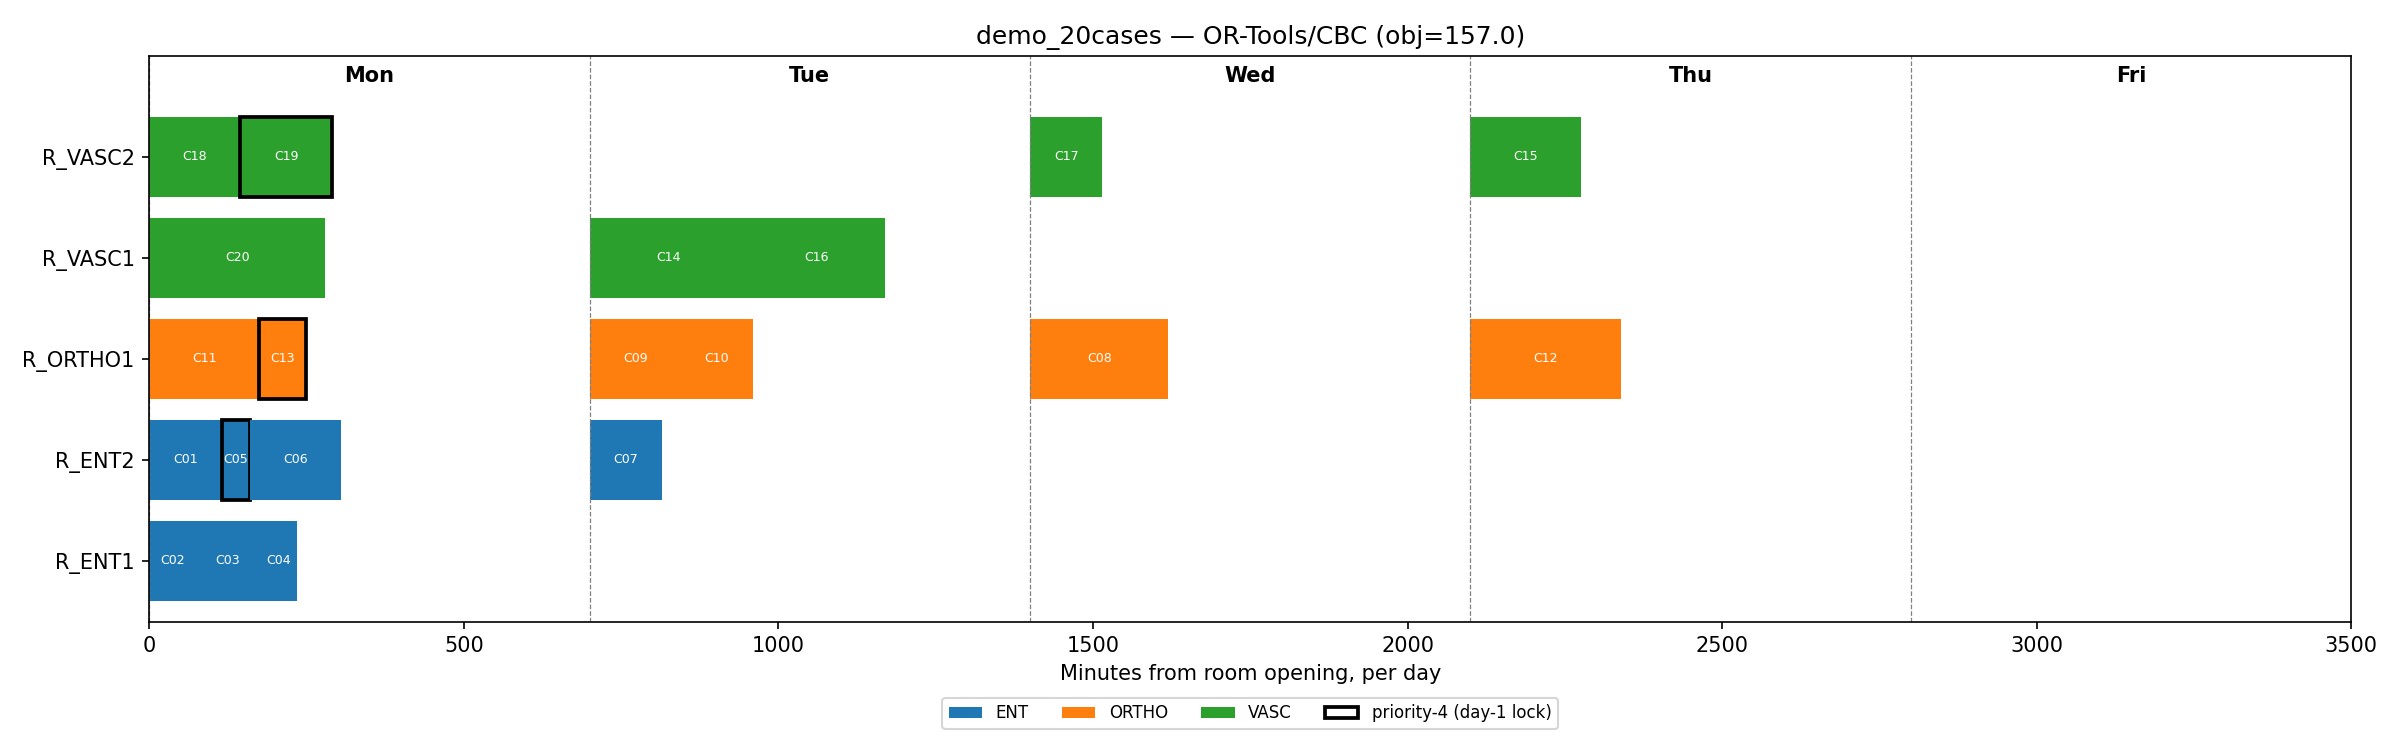
\includegraphics[width=\textwidth]{img/demo_baseline_milp.png}
  \footnotesize Same cases, no exact clock times (the MILP doesn't model any) --
  cases within a room-day are laid out back-to-back, arbitrary order.
\end{frame}

\begin{frame}{Medium Instance (200 cases) -- Primary CP-SAT Model}
  \centering
  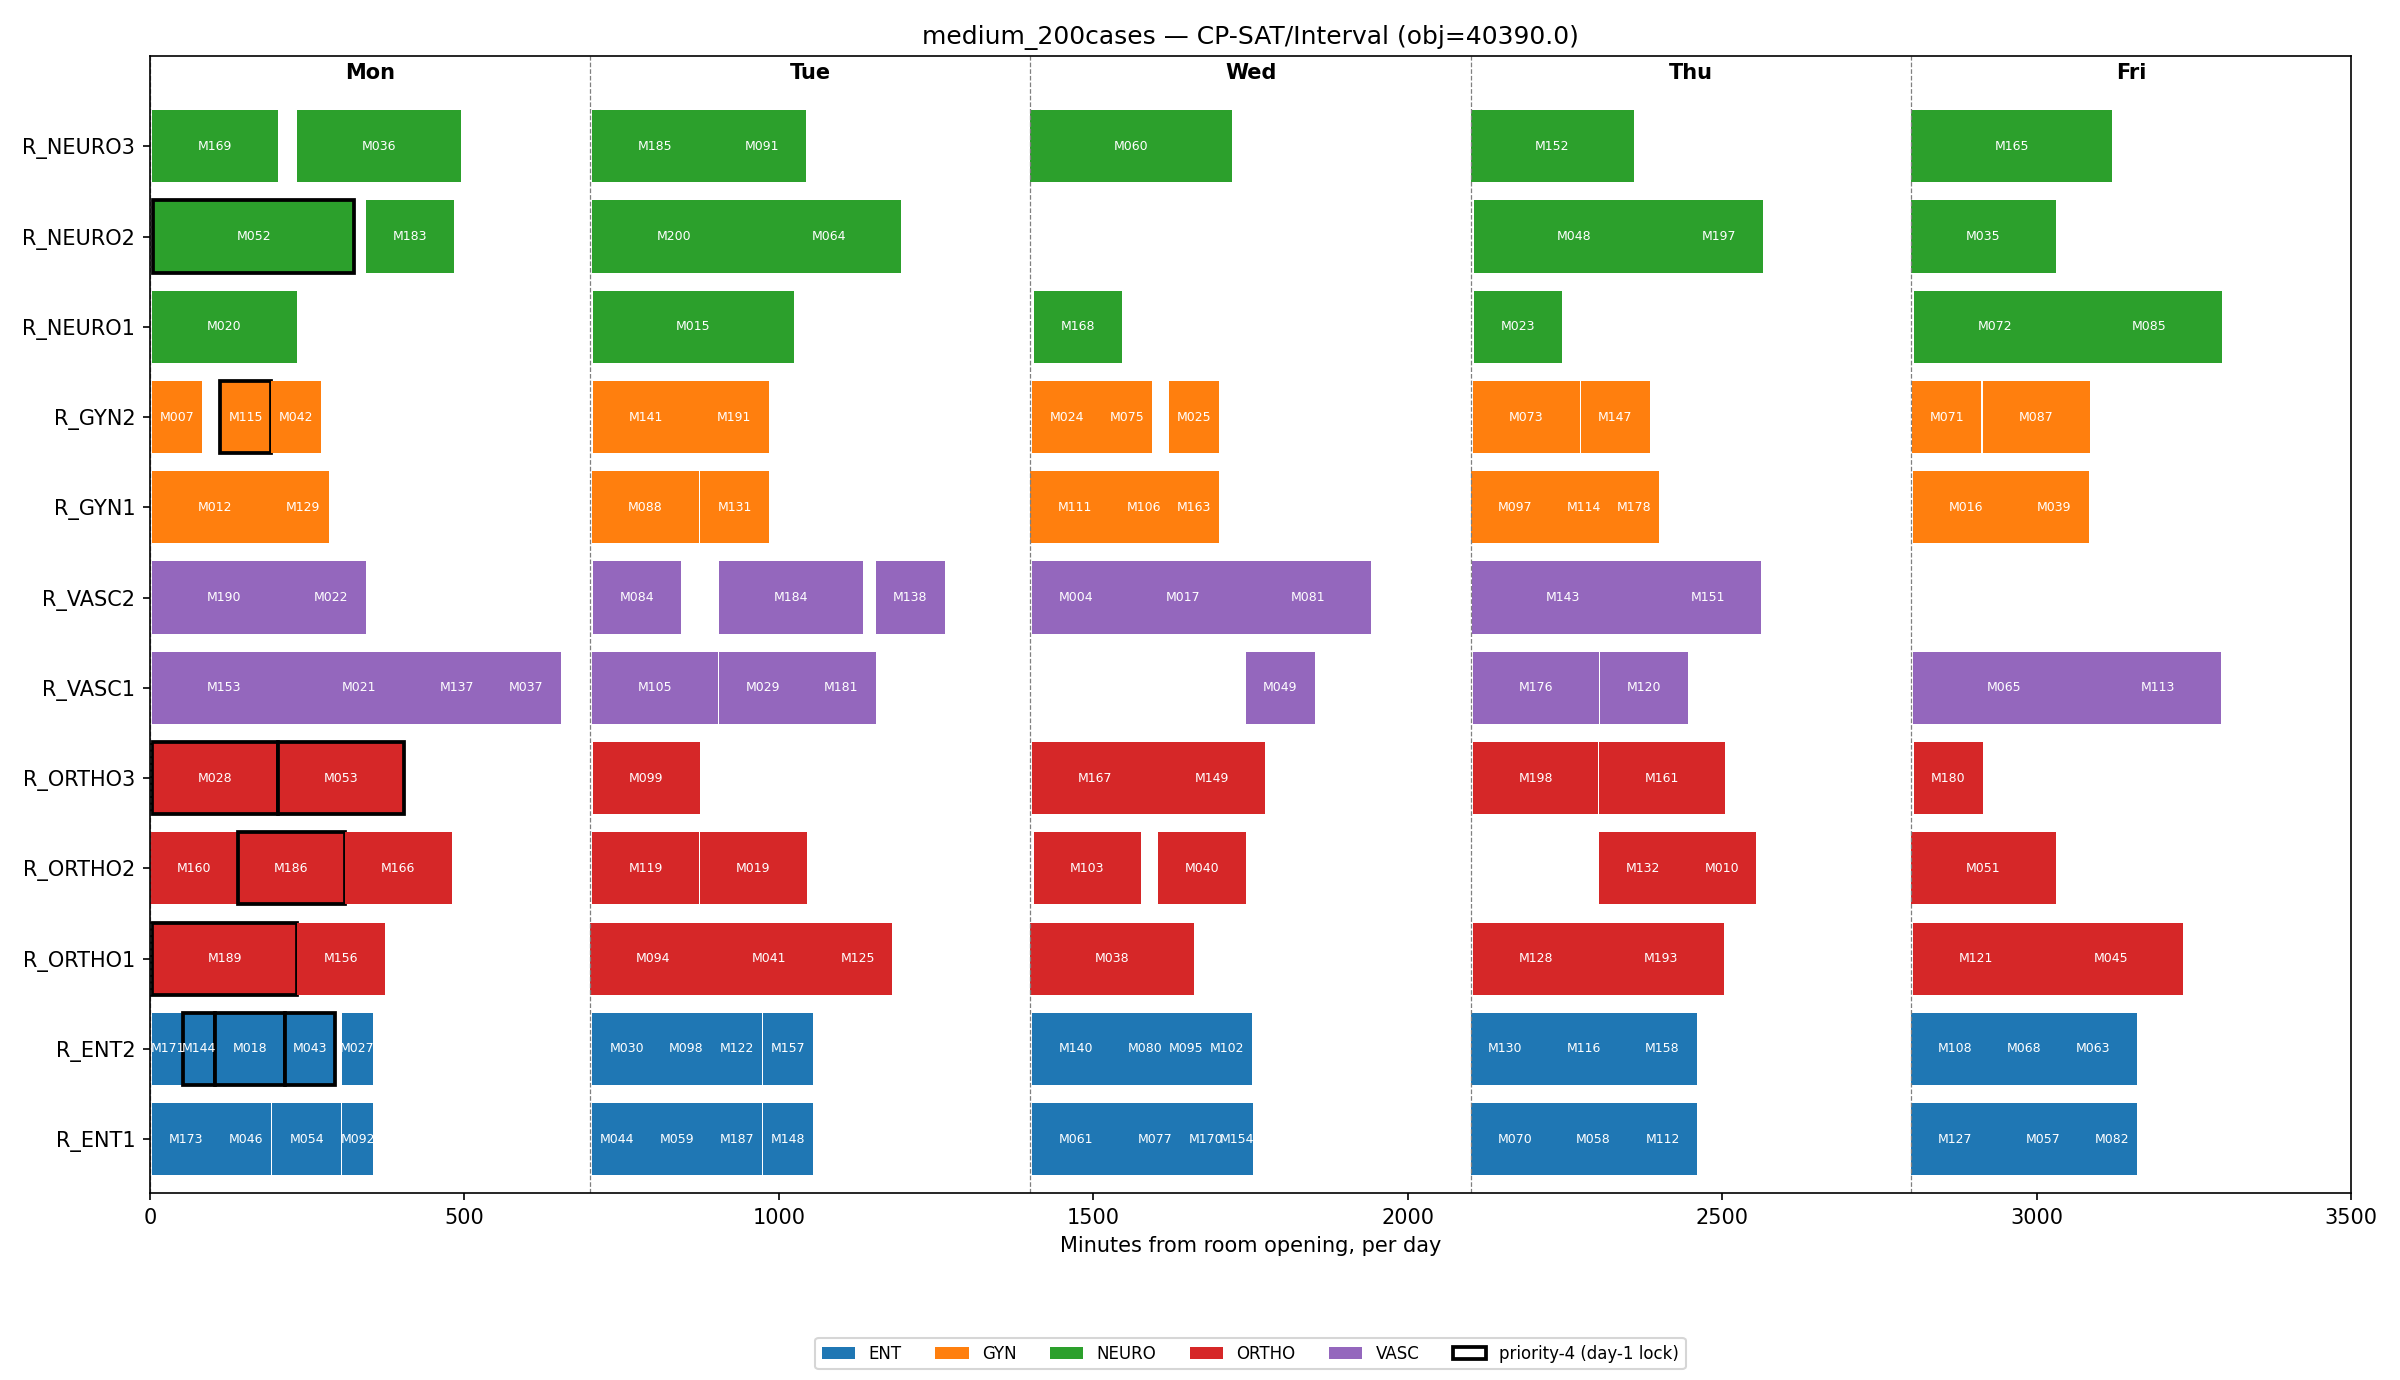
\includegraphics[width=0.85\textwidth]{img/medium_cp_sat.png}
  \footnotesize Exact per-case start times across all 12 rooms, 5 services.
\end{frame}

% ============================================================================
\section{Real-World Validation}
% ============================================================================

\begin{frame}{Testing Against Real and Literature Data}
  \footnotesize \texttt{demo\_instance()}/\texttt{medium\_instance()} are synthetic,
  literature-\emph{structured} (Cardoen et al., 2010). A third instance,
  \texttt{literature\_chln\_instance()}, is literature-\emph{calibrated}: its
  waiting-time generator reproduces, by construction, the published 2016 CHLN audit
  statistics (Marques \& Captivo, 2015) -- $\sim$16\% of cases overdue hospital-wide,
  $\sim$147 days average breach, Neurosurgery specifically $\sim$261 days. (Honestly
  noted: any one finite draw, including the shipped seed, deviates from these targets
  by sampling noise -- itself realistic.)
  \vfill
  \textbf{For testing against real hospital OR logs at full scale}, two CC BY-4.0
  datasets are a direct structural fit (same weekly horizon, same master-roster
  concept):
  \begin{itemize}
    \item Akbarzadeh \& Maenhout (2023). \emph{Real life data for operating room
      scheduling problem} -- Ghent University Hospital, May 2017. Mendeley Data,
      \href{https://data.mendeley.com/datasets/n2v49z2vnp/2}{10.17632/n2v49z2vnp.2}.
    \item Akbarzadeh \& Maenhout (2023). \emph{RealLife operating room scheduling
      dataset, 2021-Jan-May} -- 20 weekly instances. Mendeley Data,
      \href{https://data.mendeley.com/datasets/c8d342266x/1}{10.17632/c8d342266x.1}.
  \end{itemize}
  A loader is the natural next step before a real pilot -- intentionally not built
  here, per this being a small demo, not a production deployment.
\end{frame}

% ============================================================================
\section{Open Questions}
% ============================================================================

\begin{frame}{Q1 -- Passing the Torch}
  \small I'd hand a developer four things, not just the math:
  \begin{enumerate}
    \item \textbf{FORMULATION.md + \texttt{types.py}} -- the dataclasses
      \emph{are} the data dictionary; sets/parameters map 1:1 to fields.
    \item \textbf{The solver code itself} -- every constraint is labeled (C1\ldots C11)
      and the matching code carries the same label. Read side by side, no ambiguity
      about which line implements which formula.
    \item \textbf{\texttt{test\_model.py} as the acceptance contract} -- any
      reimplementation must pass the same hard-constraint checks on the same demo
      instance; I'd ask for a test per new constraint before writing the constraint.
    \item \textbf{A short glossary} of the handful of non-obvious domain terms (room
      roster, ambulatory, priority tiers). Most miscommunication on these projects is
      vocabulary, not math.
  \end{enumerate}
\end{frame}

\begin{frame}{Q2 -- A Library of Models}
  \small Four layers, solver-agnostic except the bottom one:
  \begin{enumerate}
    \item Core data abstractions -- typed dataclasses, no solver imports.
    \item Reusable constraint \emph{patterns} (capacity-sum, NoOverlap,
      tiered-priority tardiness, eligibility pre-filter) that recur across
      scheduling problems -- nurse rostering and bed allocation need the same
      shapes, not the same model.
    \item Problem templates that compose those patterns -- this repo's model is one
      such template.
    \item A thin solver-adapter layer, one file per backend family (MILP, CP, local
      search), so a new problem picks a backend without rewriting how constraints
      are expressed.
  \end{enumerate}
  \vfill
  The CP-vs-MILP comparison this deck demonstrates is itself a template for that last
  layer: justify the backend choice from the problem's structure first, verify it
  empirically on a small instance, \emph{then} commit -- rather than defaulting to
  whichever backend is most familiar.
\end{frame}

% ============================================================================
\section{Roadmap}
% ============================================================================

\begin{frame}{Extensions and Future Work}
  \footnotesize
  \begin{table}
    \centering
    \begin{tabular}{p{3.6cm}p{7.8cm}}
      \toprule
      Extension & Approach \\
      \midrule
      Stochastic durations & Two-stage stochastic program: first stage selects/places
        cases, second stage absorbs duration realisations via overtime or case bump \\
      Real-time rescheduling & Large Neighbourhood Search seeded from the current
        schedule, for same-day disruptions -- Hexaly's local-search engine is a
        natural fit \\
      Nurse/anaesthetist rostering & Extend $H$ to support staff; same NoOverlap/sum
        pattern as surgeons \\
      Multi-week rolling horizon & Solve weekly; carry forward unscheduled cases with
        increased priority weight \\
      Day-varying bed capacity & Replace the constant $\beta_\rho$ with a per-day
        \texttt{Cumulative} or reservoir decomposition \\
      \bottomrule
    \end{tabular}
  \end{table}
\end{frame}

\begin{frame}{References}
  \tiny
  \begin{enumerate}
    \item Cardoen, B., Demeulemeester, E., \& Beli\"en, J. (2010). Operating room
      planning and scheduling: A literature review. \emph{EJOR}, 201(3), 921--932.
    \item Marques, I., \& Captivo, M.E. (2015). \emph{Planeamento de cirurgias
      eletivas no Centro Hospitalar Lisboa Norte}. MSc thesis, Universidade de
      Lisboa.
    \item Denton, B.T., Miller, A.J., Balasubramanian, H.J., \& Huschka, T.R. (2010).
      Optimal allocation of surgery blocks to operating rooms under uncertainty.
      \emph{Operations Research}, 58(4), 802--816.
    \item SIGIC -- Sistema Integrado de Gest\~ao de Inscritos para Cirurgia,
      Portaria n.\textsuperscript{o} 45/2008, Di\'ario da Rep\'ublica, Portugal.
    \item Akbarzadeh, B., \& Maenhout, B. (2023). Real life data for operating room
      scheduling problem [Data set]. Mendeley Data, V2.
      \url{https://doi.org/10.17632/n2v49z2vnp.2}
    \item Akbarzadeh, B., \& Maenhout, B. (2023). RealLife operating room scheduling
      dataset, 2021-Jan-May [Data set]. Mendeley Data, V1.
      \url{https://doi.org/10.17632/c8d342266x.1}
    \item Perron, L., \& Furnon, V. \emph{CP-SAT: a Constraint Programming Solver}
      (Google OR-Tools documentation). \url{https://developers.google.com/optimization/cp}
    \item Baptiste, P., Le Pape, C., \& Nuijten, W. (2001). \emph{Constraint-Based
      Scheduling}. Kluwer Academic Publishers.
    \item Vil\'im, P. (2004). $O(n\log n)$ filtering algorithms for unary resource
      constraint. \emph{CPAIOR 2004}.
    \item Schutt, A., Feydy, T., Stuckey, P.J., \& Wallace, M.G. (2009). Why
      cumulative decomposition is not as bad as it sounds. \emph{CP 2009}.
  \end{enumerate}
\end{frame}

\begin{frame}
  \centering
  \Huge Thank You
  \vfill
  \normalsize Repository: \texttt{FORMULATION.md} $\cdot$
  \texttt{RESULTS.md} $\cdot$ \texttt{README.md}
  \vfill
  \texttt{python main.py}\quad(primary model)\qquad
  \texttt{python main.py --benchmark}\quad(comparison)
\end{frame}

\end{document}
